\documentclass{article}
\usepackage{a4wide}
\usepackage{graphicx}
\usepackage{amsmath, amsthm, amssymb}

\usepackage[utf8]{inputenc}
\usepackage{ngerman}
\usepackage{url}
\usepackage[ruled,vlined]{algorithm2e}
\usepackage[]{hyperref}
\usepackage{listings}
\usepackage{dsfont}

\newtheorem{thm}{Theorem}[section]
\newtheorem{cor}[thm]{Korollar}
\newtheorem{lem}[thm]{Lemma}
\newtheorem{defi}[thm]{Definition}
\newtheorem{definition}{Definition}
\newcounter{Chapcounter}
\newcommand\showmycounter{\addtocounter{Chapcounter}{1}\themycounter}
\newcommand{\chapter}[1] 
{ {\centering          
  \addtocounter{Chapcounter}{1} \Large \underline{\textbf{ \color{blue} Chapter \theChapcounter: ~#1}} }   
  \addcontentsline{toc}{section}{ \color{blue} Chapter:~\theChapcounter~~ #1}    
}
\hypersetup{colorlinks=true}
\hypersetup{linkcolor=black}
\usepackage{listings}
\lstdefinelanguage{Pseudo}{
  morekeywords={forall,if,then,else,return,while,do,for,DFS},
  sensitive=false,
  morecomment=[l]{//},
  morestring=[b]"
}



\setcounter{tocdepth}{4}

\begin{document}
\title{Statistische und Stochastische grundlagen der Informatik}
\date{Wintersemester 2025/26}
\author{Universität Stuttgart}
\maketitle
\tableofcontents
\newpage


\chapter{Stochastic}

\section{Introduction}
\subsection{Bertrands Paradox}
This paradox poses a nice introduction of how homogenous sampling is key for good analysis

Lets take a circle of radius 1. We trace a line that crosses the circle at some point. What is the possibility of the length of the inscribed line being $l > \sqrt{3}$? 

\textbf{Note}: $\sqrt{3}$ is the length of the size of the maximum possible triangle inscribed in the circle.

\subsubsection{First Computation: }We can imagine that the line is always paralel to the y-Axis by just rotating the axis. The intersection with the x-Axis must then be between -1 and 1. For $l = \sqrt{3}$ is $x_0 = \pm \frac{1}{2}$. So the possibility is $|x_0| > \frac{1}{2} = \frac{1}{2}$

\subsubsection{Second Computation: }Lets fix one of the intersection points with the circle $p_1$.  The angle between the line and the tangent of the circle $p_1$ will be called $\Theta$, which will be between 0 and $\pi$  radians.
For $l = \sqrt{3}$, $\Theta = \frac{\pi}{2} \pm \frac{\pi}{6}$ so the possibility of $l > \sqrt{3}$ is $\frac{\pi}{3} < \Theta <  \frac{2\pi}{3} = \frac{1}{3}$

\subsubsection{Third Computation:}  
Pick a point $p_m \neq (0,0)$ uniformly at random somewhere inside the circle.  
Now consider the chord that is perpendicular to the line connecting $p_m$ with the origin.  
This construction gives a unique chord for each interior point, and its length depends only on the distance of $p_m$ from the center.

The chord is longer than $\sqrt{3}$ exactly when the point $p_m$ lies closer than $\tfrac{1}{2}$ to the origin (this follows from the same geometry used in the first computation).  

So the probability is simply the ratio of the area of the circle of radius $1/2$ to the area of the full unit circle:
\[
\frac{\pi (1/2)^2}{\pi (1)^2} = \frac{1}{4}.
\]\section{Probability Spaces}

A probability space (or \emph{P-space}) consists of the following components:

\begin{enumerate}
    \item \textbf{Sample Space} $\Omega$:  
    A non-empty set of all possible outcomes of a random experiment  
    (e.g., the face values of a die, or the chords considered in Example 2.1).

    \item \textbf{Event System} $\mathcal{A}$:  
    A collection of subsets of $\Omega$.  
    The sets $A \in \mathcal{A}$ are called \emph{events}  
    (e.g., all even die rolls, or all chords longer than $\sqrt{3}$).

    \item \textbf{Probability Measure} $P : \mathcal{A} \to \mathbb{R}$:  
    Assigns a probability to every event.
\end{enumerate}

The model does \emph{not} contain “randomness” itself.  
In probability theory we study properties of a given probability measure $P$, 
typically using tools such as random variables and expectations, often combined with combinatorics.  
Where the probability distribution $P$ comes from, and what its results mean, belongs to the 
\emph{modeling} outside of probability theory.

Events are sets, so all usual set operations also apply here.  
In the context of events, they are interpreted as follows:

\begin{itemize}
    \item $A \cap B$: both events $A$ and $B$ occur
    \item $A \cup B$: at least one of the events $A$ or $B$ occurs
    \item $B \setminus A$: $B$ occurs but $A$ does not
    \item $A^c := \Omega \setminus A$: $A$ does not occur
\end{itemize}

Later we will require that the event system $\mathcal{A}$ is 
closed under these operations, so the result of any such operation is again an event.  
We also require that $\varnothing$ and $\Omega$ are included in $\mathcal{A}$.  
Here, $\varnothing$ is the \emph{impossible} event, and $\Omega$ is the \emph{certain} event.  
Events of the form $\{\omega\}$ with $\omega \in \Omega$ are called \emph{elementary events}.

\begin{definition}[Incompatibility]
Two events $A$ and $B$ are called \emph{incompatible} (or \emph{disjoint}) 
if $A \cap B = \varnothing$.
\end{definition}

For unions of disjoint sets we introduce a summation notation.

\begin{definition}
For pairwise disjoint sets $A_1, \ldots, A_n$ (i.e.\ $A_i \cap A_j = \varnothing$ for $i \ne j$), define:
\[
A_1 + A_2 := A_1 \cup A_2,
\]
and more generally
\[
\sum_{i=1}^n A_i := \bigcup_{i=1}^n A_i.
\]
\end{definition}
\section{Properties of Probability Computation}

\[
\mathbb{P}(\emptyset) = 0
\]
\[
\mathbb{P}(\Omega) = 1
\]
\[
\forall A \subset \Omega : \mathbb{P}(A) \ge 0,\quad \mathbb{P}(A) \le 1
\]
\[
\mathbb{P}(A \cup B) = \mathbb{P}(A) + \mathbb{P}(B)
\quad \text{for disjoint } A,B.
\]

For independent events:
\[
\mathbb{P}\!\left(\bigcap_{i=1}^n A_i\right)
= \prod_{i=1}^n \mathbb{P}(A_i).
\]

\section{Random Variables}

A key tool for describing probability spaces are \emph{random variables}.

\begin{definition}[Random Variable]
A random variable on a probability space is a function
\[
X : \Omega \to \mathbb{R}.
\]
(We will slightly refine this definition later in Section~6.)
\end{definition}

Random variables allow us to extract numerical properties of outcomes.  
For example, when rolling a die twice, the sample space is
\[
\Omega = \{1, \dots, 6\}^2,
\]
and the sum of both dice is the random variable
\[
X(w_1, w_2) := w_1 + w_2.
\]

Often we are interested in the preimage of a set $A \subset \mathbb{R}$:
\[
X^{-1}(A) := \{ \omega \in \Omega : X(\omega) \in A \}.
\]

For the example above,
\[
X^{-1}([3,4])
= \{ (1,2), (1,3), (2,1), (2,2), (3,1) \}.
\]

It is common (though somewhat sloppy) to write these sets in shorthand, e.g.
\[
\{3 \le X \le 4\} := X^{-1}([3,4]).
\]

For the probability space we are considering here, the following holds:
\[
\{3 \le X \le 4\} = \{X = 3\} \cup \{X = 4\}.
\]

A random variable always maps into $\mathbb{R}$, so all normal algebraic 
operations apply, and we may form expressions such as $|X|$ or $\max(X,Y)$.

\section{Finite Probability Spaces}

\subsubsection{Definition.}
A finite probability space is a pair $(\Omega,\mathbb{P})$ with
\[
\begin{cases}
  \forall A \subset \Omega : \mathbb{P}(A) \ge 0,\\[2mm]
  \mathbb{P}(\Omega) = 1,\\[2mm]
  \forall A,B \subset \Omega,\ A \cap B = \emptyset :
  \mathbb{P}(A \cup B) = \mathbb{P}(A) + \mathbb{P}(B).
\end{cases}
\]

Because we can write an event $A$ as
\[
A = \sum_{w\in A}\{w\},
\]
it is enough to define $\mathbb{P}$ on singletons via a probability function
\[
p : \Omega \to [0,1],
\]
with
\[
\sum_{w\in \Omega} p(w) = 1,
\qquad
\mathbb{P}(A) = \sum_{w\in A} p(w).
\]

\subsection{Probability Function of a Random Variable}

We define
\[
\mathbb{P}^X : \mathcal{P}(X(\Omega)) \to \mathbb{R},
\qquad
\mathbb{P}^X(B) := \mathbb{P}(X^{-1}(B)).
\]

\[
\mathbb{P}(X = x) := \mathbb{P}(X^{-1}(\{x\})),
\qquad
\mathbb{P}(a \le X \le b) := \mathbb{P}(X^{-1}([a,b])).
\]

\subsection{Distribution Function of a Random Variable}

\[
F^X : \mathbb{R} \to \mathbb{R},\qquad
F^X(x) := \mathbb{P}(X \le x).
\]

With the properties:
\[
\lim_{x\to -\infty} F^X(x) = 0,
\qquad
\lim_{x\to \infty} F^X(x) = 1.
\]

\subsubsection{Example.}
An example of such a probability space is the throwing of a die.

\section{Laplace Experiments}

Often all elements $w \in \Omega$ have the same elementary probability:
\[
\forall w \in \Omega : p(w) = \frac{1}{|\Omega|}.
\]
Thus,
\[
\forall A \subset \Omega : \mathbb{P}(A) = \frac{|A|}{|\Omega|}.
\]

Such probability spaces are called \textbf{Laplace probability spaces}, and 
$\mathbb{P}$ is a discrete uniform distribution.

\section{Expected Value}

For a random variable $X$ we define the expected value as
\[
\mathbb{E}(X) := \sum_{w\in \Omega} X(w)\,\mathbb{P}(\{w\})
= \sum_{x\in X(\Omega)} x\,\mathbb{P}(X = x).
\]

\subsection{Properties of the Expected Value}

\subsubsection{Linearity.}
\[
\mathbb{E}\!\left(\sum_{i=1}^n \alpha_i X_i\right)
= \sum_{i=1}^n \alpha_i\, \mathbb{E}(X_i).
\]

\subsubsection{Expected Value of the Indicator Function.}
If we define
\[
\mathds{1}_A(x) =
\begin{cases}
1 & x \in A,\\
0 & x \notin A,
\end{cases}
\]
then
\[
\mathbb{E}(\mathds{1}_A) = \mathbb{P}(A).
\]

\subsubsection{Monotonicity.}
\[
(\forall w\in\Omega : X(w) \le Y(w))
\ \Rightarrow\ 
\mathbb{E}(X) \le \mathbb{E}(Y).
\]

\subsubsection{Transformation Rule.}
For a random variable $X$ and a function $g:\mathbb{R} \to \mathbb{R}$,
let $g(X)(w) := g(X(w))$. Then
\[
\mathbb{E}(g(X))
= \sum_{x\in X(\Omega)} g(x)\,\mathbb{P}(X = x).
\]

\section{Variance}

For a finite probability space $(\Omega,\mathbb{P})$ and a random variable $X$ we define
\[
\mathbb{V}(X) := \mathbb{E}\bigl((X - \mathbb{E}(X))^2\bigr)
\]
as the variance of $X$.

\[
\sigma(X) := \sqrt{\mathbb{V}(X)}
\]
is called the standard deviation.


\chapter{Statistic}
\textbf{ADD TYPES OF STATISTIC}

\section{Basic Concepts -- German-English Translation}
\begin{itemize}
  \item \textbf{Statistische Einheit:} Objects that are analyzed
  \item \textbf{Grundgesamtheit:} Population under study
  \item \textbf{Teilgesamtheit:} Subset of the population
  \item \textbf{Stichprobe:} Sample
  \item \textbf{Merkmal / Variable:} Property we are observing
  \item \textbf{Ausprägung / Wert:} The value of the property for a specific object
  \item \textbf{Kenngröße:} Parameter
  \item \textbf{Urliste:} Raw Data Set. The unconverted data before processing
\end{itemize}

The properties (\textit{Merkmale}) we analyze can have different characteristics:
\begin{itemize}
  \item \textbf{Discrete:} Countable number of values
  \item \textbf{Continuous (stetig):} All possible values within an interval
  \item \textbf{Quasi-Continuous (quasi-stetig):} Continuous but cannot be measured exactly
\end{itemize}

These properties also have different scales (\textit{Skala}):
\begin{itemize}
  \item \textbf{Nominalskala:} Names, categories, etc.
  \item \textbf{Ordinalskala:} Values have a defined order, but distances between values are not meaningful
  \item \textbf{Kardinalskala:} Measurable, metric scale
\end{itemize}

\section{Data Collection}
\subsection{Experiment}
Obtaining data by actively interacting with the environment under study. Not always possible due to laws or constraints.

\subsection{Erhebung (Data Collection)}
Usually surveys or observations. Does not interact directly with the environment, less affected by external constraints.

Multiple types:
\begin{itemize}
  \item \textbf{Primärstatistisch:} Data collected directly from the environment
  \item \textbf{Sekundärstatistisch:} Data collected based on existing primary data
  \item \textbf{Tertiärstatistisch:} Data based on transformed or compressed existing data
\end{itemize}

\textbf{Vollerhebung:} Data collection on the complete population

\textbf{Important:} Avoid bias.

\subsubsection{Vollerhebung vs Stichprobe} When sampling, pay attention to how the sample is drawn.

\section{Study Designs (\textit{Studiendesigns})}
\begin{itemize}
  \item \textbf{Querschnittsstudie:} Analysis of multiple objects at a specific time point
  \item \textbf{Zeitreihe:} Analysis of one object over time
  \item \textbf{Längsschnittsstudie:} Analysis of multiple objects over time
\end{itemize}

\section{Univariable Descriptive and Explorative Statistics}
\subsection{First Parameter (\textit{Kenngröße}) -- Frequency}

If we define a set of $n$ data points where the property $X$ is observed:
\[
x_1, \dots, x_n
\]

Let the possible encountered values of $X$ (ordered) be:
\[
a_1, \dots, a_k, \quad k \leq n
\]

We can define the following:
\begin{itemize}
  \item $h(a_j) = h_j$, frequency of $a_j$ in $X$. \textbf{Absolute Frequency}
  \item $f(a_j) = f_j = \frac{h_j}{n}$, \textbf{Relative Frequency}
  \item $h_1, \dots, h_k$, \textbf{Absolute Frequency Distribution}, displayed through a histogram
  \item $f_1, \dots, f_k$, \textbf{Relative Frequency Distribution}
\end{itemize}

\subsubsection{Classification} The number of classes $k$ can be computed as:
\[
k = \lfloor \sqrt{n} \rfloor \quad \text{for } n \leq 100
\]

or, for larger $n$:
\[
k = \lfloor 10 \cdot \log_{10}{n} \rfloor
\]
\subsection{Characterization over form parameters}
We can classify a distribution on its amount of peaks, if its symetric and basically the form of the graph

\subsection{Characterization over empirical distribution function}
ONLY FOR ORDINAL SCALED DATA

We can define the following

\textbf{Absolute Cumulative Frequency Distribution}
  \[H(x) = h(a_1)+ h(a_2) + ..+h(a_j) = \sum_{i:a_i\leq x}h_i\]

  \textbf{Empirical Distribution Function}
  \[F(x) = f(a_1)+ f(a_2) + ..+f(a_j) = \sum_{i:a_i\leq x}f_i\]

  This characterization answers the question of: what percentage of the data is $\leq x$?

  Doesnt answer: Where is the center of the data...

\subsection{Characterization over Central tendency}

\subsubsection{Central tendency (Lagemaße)}

This concept describes the center of a distribution through a numerical value

\subsubsection{Definition. Central tendency: }Its a function
\[L : \mathbb{R}^n \to \mathbb{R}\] with the following property
\[L(x_1 + a , ... , x_n +a ) = L (x_1,...,x_n) + a \text{    } ,  \forall a,x_1,...,x_n \in \mathbb{R}\]

The most used central tendency is the arithmetical mean.


\subsubsection{Arithmetical Mean: } Given the image list $x_1,...,x_n$. We can compute the arithmetical mean as follows

\[\overline{x} = \frac{1}{n}(x_1+...+x_n) = \frac{1}{n} \sum_{i=1}^{n}x_i\]

\subsubsection{Median: }
If we define this list as sorted $(x_{(1)},...x_{(n)})$, the median is the middle point
\[x_{med}\begin{cases}
  x_{(\frac{n+1}{2})} & \text{ if n odd}\\
  \frac{x_{(n/2)}  + x_{(n/2 + 1)}}{2} & \text{ else}\\
\end{cases}\]


\subsubsection{Mode: }
The most common element

\subsubsection{Geometrical Middle (midpoint): }Given a list $x_1,...,x_n$
\[x_{geom} = (x_1\cdot ... \cdot x_n)^{\frac{1}{n}} = (\prod_{i=1}^{n}x_i)^\frac{1}{n}\]

\subsubsection{Harmonical Middle: }Given a list $x_1,...,x_n$
\[ x_{harm} = \frac{1}{\frac{1}{n} \sum_{i=1}^n \frac{1}{x_i}}\]

\subsection{Characterization over Statistical Dispersion}

\subsubsection{Statistical dispersion (Streuungsmaße)}

\subsubsection{Definition: }Its a function
\[S : \mathbb{R}^n \to \mathbb{R}\] with the following property
\[S(x_1 + a , ... , x_n +a ) = S(x_1,...,x_n)  \text{    } ,  \forall a,x_1,...,x_n \in \mathbb{R}\]

\subsubsection{Variation width, sample space width}: $ = x_{max} - x_{min}$

\subsection{p-Quantil (Percentil)}
Given a list of ordered data
\[x_1 \leq x_2 \leq \dots \leq x_n \]
We can define  $x_p$ with $0 < p < 1$
as the value that splits the ordered list from above into two parts so that

\[\frac{|\{x_i : x_i \leq x_p\}|}{n} \geq p \]

and 
\[\frac{|\{x_i : x_i \geq x_p\}|}{n} \geq 1-p \]

Basically: The hypothetical value that splits the list in two pieces, the left piece taking p\% of the total values

\[x_p = F^{-1}(p)\]


Its similar to the z quantils but with discrete data

\subsection{Interquantilerange (Interquartilsabstand)}
We define
\[d_Q = x_{0.75} - x_{0.25}\]

In general, the following 5-Point description is pretty helpful to imagine a distribution

\[x_{min},x_{0.25},x_{median},x_{0.75},x_{max}\]

\subsection{Graphical display}
\subsubsection{Box Plot: }If we draw all the points of the distribution on a line. The box plot is drawn as follows (image describes both in expanded box plot)

\subsubsection{Expanded Box Plot: } Same as box plot just with the fence.

The fence is computed as $\{x_{0.25} - 1.5 \cdot d_Q,x_{0.75} + 1.5 \cdot d_Q\}$ 
If the fence doesnt land on any point, we \textbf{compress} it until the next point on both edges


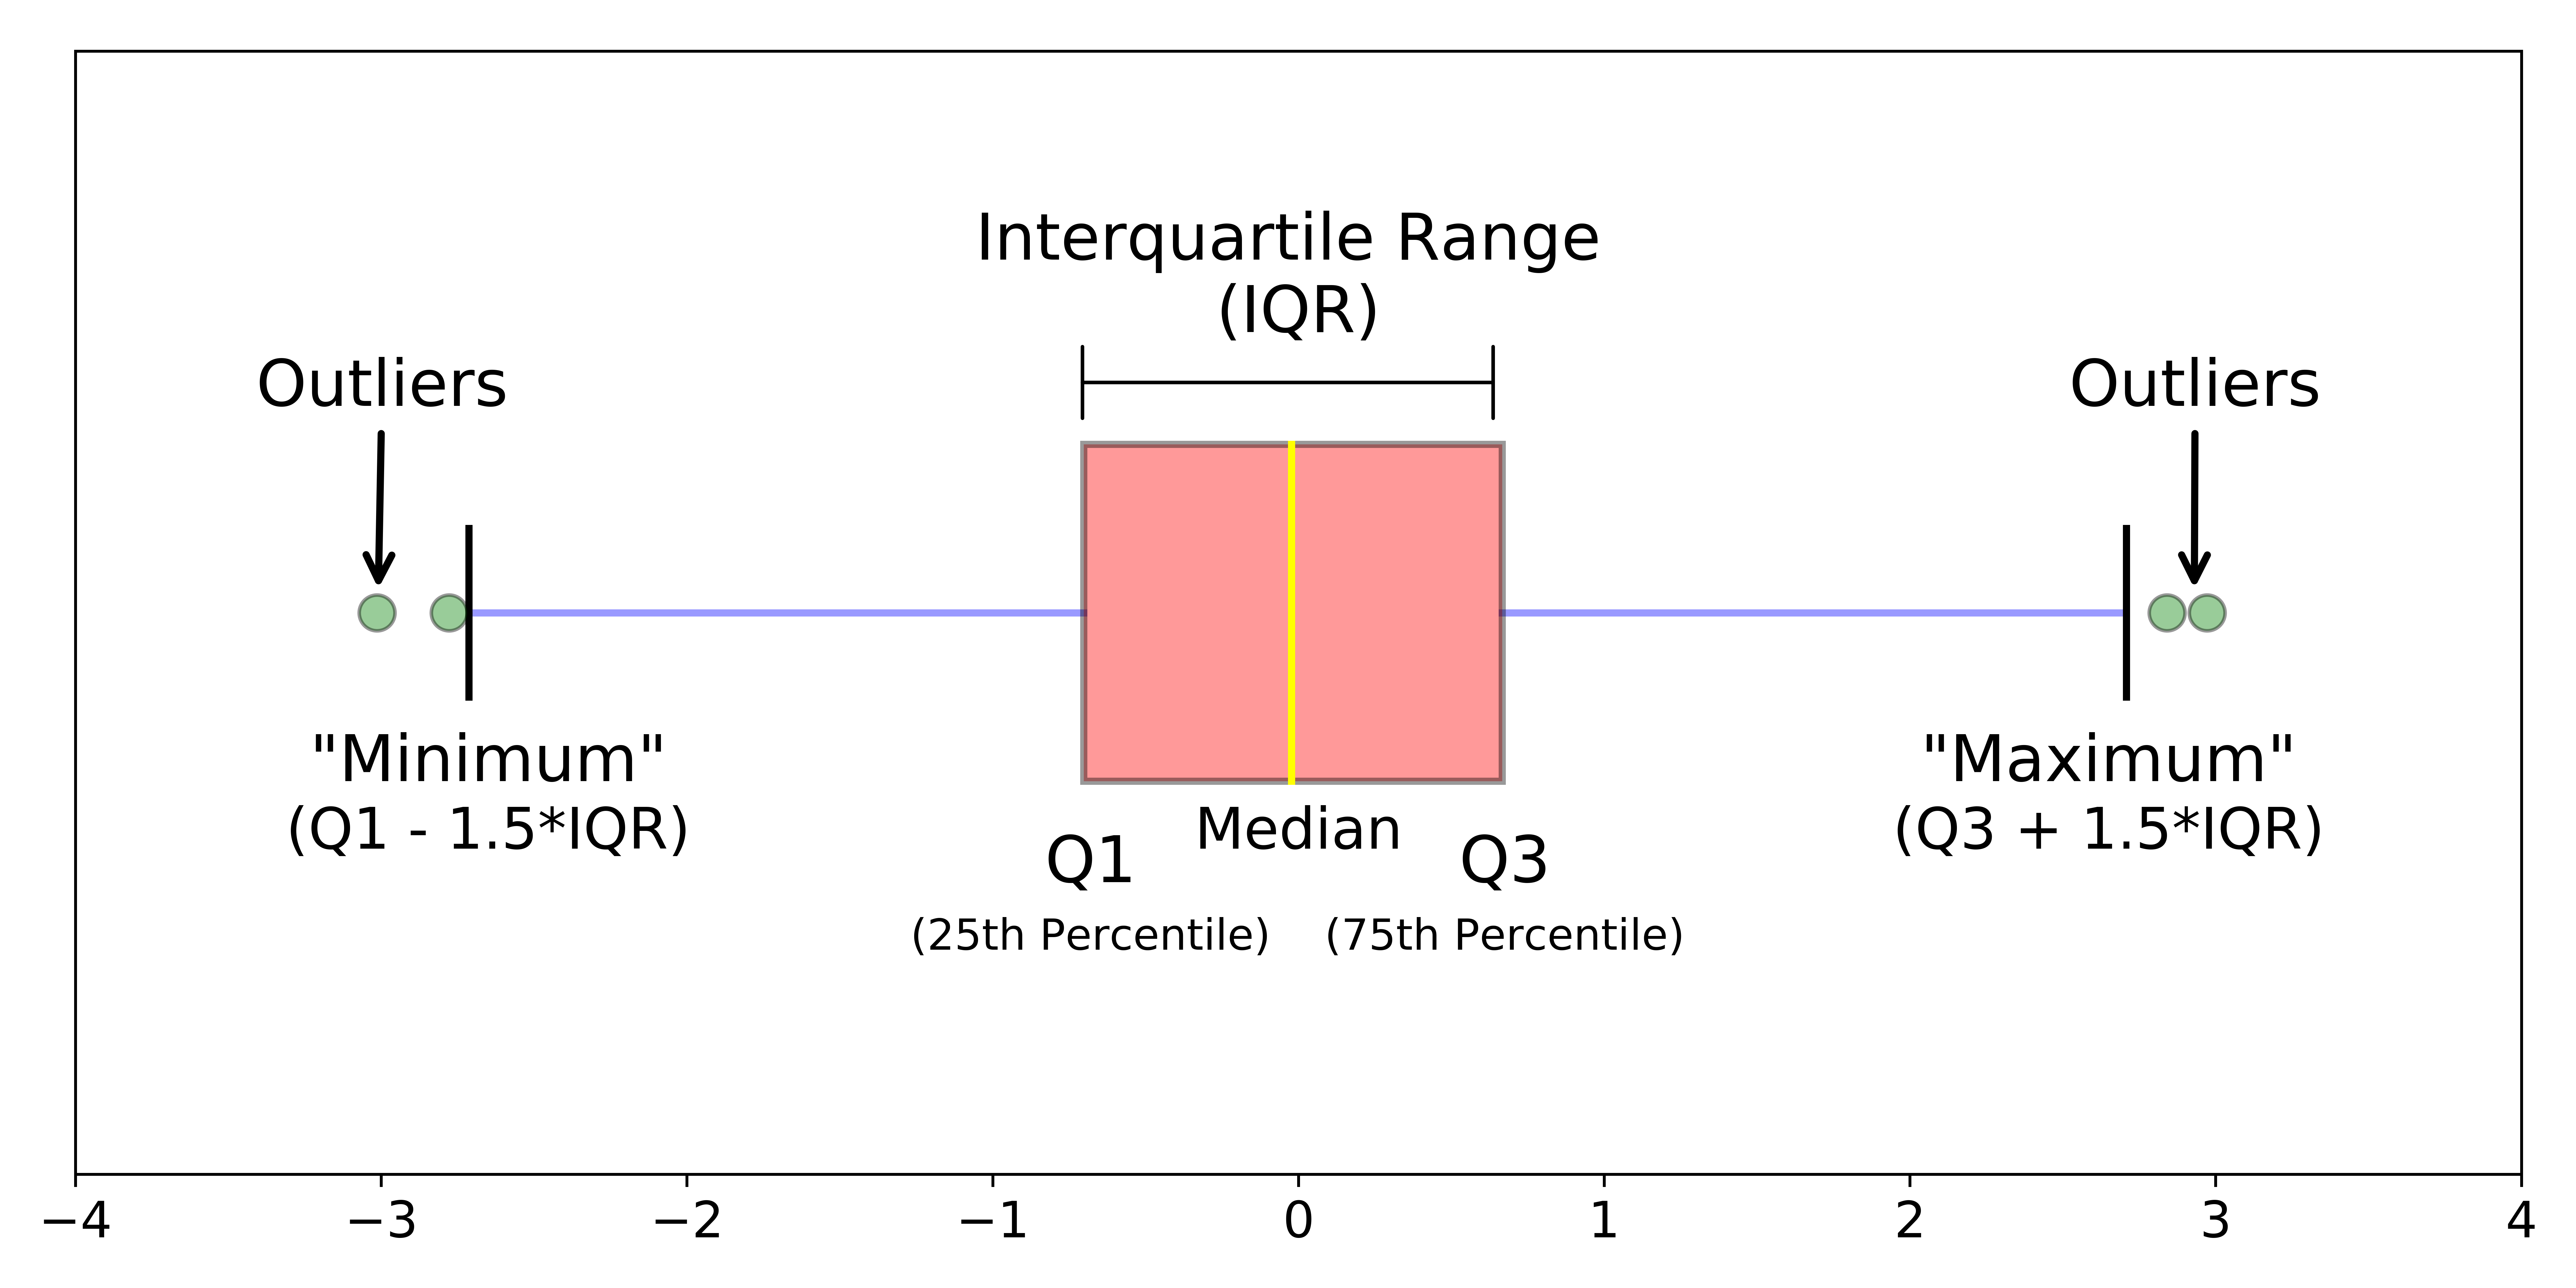
\includegraphics[scale=0.04]{assets/boxplot.png}

\subsection{Calculation rules}
\subsubsection{Transformation rule: } For a linear transformation $y = ax + b$ the following stands
\[\tilde{s}^2_y = a^2\tilde{s}^2_x\]

Note: $\tilde{s}$ will be described blow

\subsubsection{Displacement theorem: } For all $c \in \mathbb{R}$

\[\sum_{i=1}^n(x_i-c)^2 = \sum_{i=1}^n(x_i-\overline{x})^2 + n(\overline{x}-c)^2 \]

For $c = 0$

\[\tilde{s}^2  = \left(\frac{1}{n} \sum_{i=1}^n x_i^2\right) - \overline{x}^2\]


\subsection{Characterization over Form parameters (v2?)}
\subsubsection{Skewness (Schiefe)}

We can define it as 
\[g_m = \frac{\frac{1}{n} \sum_{i=1}^n(x_i - \overline{x})^3}{\tilde{s}^3}\]

This explains a bit the simmetry of the data. If $<0$ the peak is more on the right, if $=0$ more symmetric, and if $>0$ peak is more on the left

\subsubsection{Curvature (Wölbung)}

\[\gamma = \frac{\frac{1}{n} \sum_{i=1}^n(x_i - \overline{x})^4}{\tilde{s}^4} - 3\]

Talks about the pronunciation of the curvature. $=0$ represents similarity to $N(0,1)$, positive means more prominent curve upwards, negative means flatter

\subsection{Konzentrationsmaße}
Konzentrationsmaße are used to analyze inequality (unequal distribution) of values within a dataset.

\subsubsection{Lorenzkurve (Lorenz Curve)}
Given a raw dataset on a cardinal scale with non-negative values
\[
x_1 \leq x_2 \leq \dots \leq x_n,
\]
we define the traverse chain
\[
(0,0),(u_1,v_1),\dots,(u_n,v_n),
\]
where
\[
u_j = \frac{j}{n} \quad \text{(proportion of individuals)},
\]
\[
v_j = \frac{\sum_{i = 1}^{j} x_i}{\sum_{i = 1}^{n} x_i} 
\quad \text{(cumulative relative sum)}.
\]

The Lorenz curve shows the cumulative share of the total value held by the lowest $u_j$ proportion of individuals.
Perfect equality corresponds to the diagonal line $v = u$.
The stronger the downward deviation from the diagonal, the higher the inequality.

\subsubsection{Gini Coefficient}
For an ordered dataset, the Gini coefficient is defined as
\[
G = \frac{\text{Area between the diagonal and the Lorenz curve}}
{\text{Area between the diagonal and the } u\text{-axis}}
= 2 \cdot \text{Area between the diagonal and the Lorenz curve}.
\]

For discrete data:
\[
G = \frac{2\sum_{i = 1}^{n} i x_i}{n \sum_{i = 1}^{n} x_i}
- \frac{n+1}{n}.
\]

The Gini coefficient measures inequality:  
$G = 0$ indicates perfect equality, and larger values indicate stronger inequality.
The maximum value depends on the sample size $n$.

\subsubsection{Normalized Gini Coefficient}
To remove the dependence on sample size, the Gini coefficient can be normalized:
\[
G^* = \frac{G}{G_{\max}} = \frac{n}{n-1} G \in [0,1].
\]

\section{Multivariate Descriptive and Explorative Statistics}

\subsection{Contingency Table}
A contingency table summarizes the joint distribution of two variables.

Given variables $X$ and $Y$ with observed values
\[
x_1,\dots,x_k \quad \text{and} \quad y_1,\dots,y_m,
\]
the table is:

\begin{center}
\begin{tabular}{|c|c|c|c|c|}
\hline
 & $x_1$ & $\dots$ & $x_k$ & total \\
\hline
$y_1$ & & & & \\
\hline
$\vdots$ & & & & \\
\hline
$y_m$ & & & & \\
\hline
total & & & & \\
\hline
\end{tabular}
\end{center}

The table entries can be:
\begin{itemize}
\item Absolute frequencies $h_{i,j}$
\item Relative frequencies $f_{i,j}$
\end{itemize}

The row and column totals (e.g.\ $h_{\cdot,j} = \sum_{i=1}^{k} h_{i,j}$) are called \textbf{marginal frequencies}.
Their relative versions are called \textbf{relative marginal frequencies}.

\subsection{Conditional Frequencies}
The conditional frequency of $X = a_i$ given $Y = b_j$ is
\[
f_X(a_i \mid b_j) = \frac{h_{i,j}}{h_{\cdot,j}}.
\]

\subsection{Correlation Analysis in Contingency Tables}

\subsubsection{$\chi^2$ Coherence Measure}
\[
\chi^2 = \sum_{i = 1}^{k}\sum_{j=1}^{m}
\frac{(h_{i,j} - \tilde{h}_{i,j})^2}{\tilde{h}_{i,j}} \in [0,\infty),
\]
where the expected frequencies under independence are
\[
\tilde{h}_{i,j} := \frac{h_{i,\cdot} h_{\cdot,j}}{n}.
\]

\textbf{Explanation:}  
$\chi^2$ compares observed frequencies with expected frequencies assuming independence.
Large values indicate strong deviations from independence, hence statistical dependence between $X$ and $Y$.
If $\chi^2 = 0$, the variables are independent.

\subsubsection{Contingency Coefficient}
\[
K = \sqrt{\frac{\chi^2}{n + \chi^2}},
\]
with
\[
K \in \left[0, \sqrt{\frac{M-1}{M}}\right], 
\quad M = \min\{k,m\}.
\]

\subsubsection{Normalized Contingency Coefficient}
\[
K^* = \frac{K}{\sqrt{\frac{M-1}{M}}}, \quad K^* \in [0,1].
\]

The normalized coefficient allows comparison across tables of different sizes.

\subsubsection{Empirical Correlation Coefficient}

Also known as the \textbf{Bravais-Pearson correlation coefficient} or \textbf{Pearson's correlation coefficient}.

For a sample $(x_1, y_1), \ldots, (x_n, y_n)$, we define the empirical correlation coefficient as:
\[
r = \frac{\sum_{i=1}^{n}(x_i - \overline{x})(y_i - \overline{y})}{\sqrt{\sum_{i=1}^{n}(x_i - \overline{x})^2} \cdot \sqrt{\sum_{i=1}^{n}(y_i - \overline{y})^2}}
\]
where $\overline{x} = \frac{1}{n}\sum_{i=1}^{n}x_i$ and $\overline{y} = \frac{1}{n}\sum_{i=1}^{n}y_i$ are the sample means.

This can be equivalently written using sample covariance and standard deviations:
\[
r = \frac{\tilde{s}_{xy}}{\tilde{s}_x \cdot \tilde{s}_y}
\]
where $\tilde{s}_{xy} = \frac{1}{n}\sum_{i=1}^{n}(x_i - \overline{x})(y_i - \overline{y})$ is the sample covariance, and $\tilde{s}_x = \sqrt{\frac{1}{n}\sum_{i=1}^{n}(x_i - \overline{x})^2}$ and $\tilde{s}_y = \sqrt{\frac{1}{n}\sum_{i=1}^{n}(y_i - \overline{y})^2}$ are the sample standard deviations.

\textbf{Properties:}
\begin{itemize}
    \item $r \in [-1, 1]$ (the correlation coefficient is bounded)
    \item $r > 0$ indicates a positive linear correlation
    \item $r < 0$ indicates a negative linear correlation
    \item $r = 0$ indicates no linear correlation
    \item $|r| = 1$ indicates perfect linear correlation
\end{itemize}

\subsection{Linear Regression}

Linear regression is a statistical method for modeling the relationship between a dependent variable $Y$ and one or more independent variables (predictors) $X$. The goal is to find a linear equation that best describes how these variables relate.

Since real data contains measurement errors and random variation, we model the relationship as:
\[
Y = f(X) + \epsilon
\]
where $\epsilon$ represents the random error term with $\mathbb{E}[\epsilon] = 0$.

For simple linear regression with a single predictor, we assume:
\[
f(X) = \alpha + \beta X
\]
where $\alpha$ is the intercept and $\beta$ is the slope parameter.

\subsubsection{Method of Least Squares}

The method of least squares finds the estimators $\hat{\alpha}$ and $\hat{\beta}$ that minimize the sum of squared residuals. We define the objective function:
\[
Q(\alpha, \beta) = \frac{1}{n}\sum_{i=1}^{n}\epsilon_i^2 = \frac{1}{n}\sum_{i=1}^{n}(y_i - (\alpha + \beta x_i))^2
\]

Taking partial derivatives with respect to $\alpha$ and $\beta$ and setting them equal to zero yields the normal equations. The solution is:
\[
\hat{\beta} = \frac{\tilde{s}_{xy}}{\tilde{s}_x^2} = \frac{\sum_{i=1}^{n}(x_i - \overline{x})(y_i - \overline{y})}{\sum_{i=1}^{n}(x_i - \overline{x})^2}
\]
\[
\hat{\alpha} = \overline{y} - \hat{\beta}\overline{x}
\]

Note that $\hat{\beta} = r \cdot \frac{\tilde{s}_y}{\tilde{s}_x}$, showing the connection between the regression slope and the correlation coefficient.

\subsection{Residual Analysis}

Residual analysis is a technique to assess how well a regression model fits the observed data. The fitted values are $\hat{y}_i = \hat{\alpha} + \hat{\beta}x_i$, and the residuals are $e_i = y_i - \hat{y}_i$.

\subsubsection{Decomposition of Total Variation}

The total variation in the dependent variable can be decomposed as:
\[
\underbrace{\text{SST}}_{\text{Total Sum of Squares}} = \underbrace{\text{SSE}}_{\text{Explained Sum of Squares}} + \underbrace{\text{SSR}}_{\text{Residual Sum of Squares}}
\]
\[
\sum_{i=1}^{n}(y_i - \overline{y})^2 = \sum_{i=1}^{n}(\hat{y}_i - \overline{y})^2 + \sum_{i=1}^{n}(y_i - \hat{y}_i)^2
\]

This decomposition states that the total variability in $Y$ equals the variability explained by the model plus the unexplained (residual) variability.

\subsubsection{Coefficient of Determination}

The coefficient of determination, denoted $R^2$, measures the proportion of variance in the dependent variable that is explained by the independent variable(s):
\[
R^2 = \frac{\text{SSE}}{\text{SST}} = \frac{\sum_{i=1}^{n}(\hat{y}_i - \overline{y})^2}{\sum_{i=1}^{n}(y_i - \overline{y})^2} = 1 - \frac{\text{SSR}}{\text{SST}}
\]

\textbf{Properties:}
\begin{itemize}
    \item $R^2 \in [0, 1]$
    \item $R^2 = 0$ means the model explains none of the variability
    \item $R^2 = 1$ means the model explains all of the variability (perfect fit)
    \item For simple linear regression: $R^2 = r^2$ (the square of the correlation coefficient)
\end{itemize}


\subsection{Quantile-Quantile Diagrams (QQ-Plots)}

A \textbf{QQ-plot} is a graphical tool to compare two distributions by plotting their quantiles against each other.

\subsubsection{How to Build a QQ-Plot}

\begin{itemize}
    \item \textbf{X-axis:} Quantiles $x_p$ from the first distribution
    \item \textbf{Y-axis:} Quantiles $y_p$ from the second distribution
    \item Plot points $(x_p, y_p)$ for probabilities $p = 0.00, 0.05, 0.10, \ldots, 1.00$
\end{itemize}

\subsubsection{Normal QQ-Plots}

The most common use is comparing your data to a normal distribution $N(0,1)$. These are called \textbf{Normal QQ-plots} or \textbf{NQ-plots}.

\subsubsection{How to Read QQ-Plots}

\begin{itemize}
    \item \textbf{Points close to diagonal line:} Data follows the reference distribution well
    \item \textbf{Points far from diagonal:} Data doesn't match the reference distribution
    \item \textbf{Axis scaling doesn't matter:} Focus on the pattern, not the numbers
    \item \textbf{Quick visual check:} Easy way to see if your data is normally distributed
\end{itemize}

\subsection{Correlation and Causality}

\textbf{Important:} High correlation does NOT mean one variable causes the other. Correlation $\neq$ Causation.

Here are common mistakes when interpreting correlations:

\subsubsection{Spurious Correlation (Scheinkorrelation)}

Two variables are highly correlated but have no real relationship.

\textbf{Why it happens:}
\begin{itemize}
    \item A hidden third variable affects both
    \item Pure coincidence
    \item Both follow the same external trend
\end{itemize}

\textbf{Example:} Ice cream sales and drowning deaths are correlated. But ice cream doesn't cause drowning—hot weather causes both!

\subsubsection{Hidden Correlation (Verdeckte Korrelation)}

Overall data shows no correlation, but relationships exist within subgroups.

\textbf{Why it happens:} Combining different groups hides their individual patterns.

\textbf{Example:} Total tobacco consumption stays constant over time (no correlation). But when you separate by gender:
\begin{itemize}
    \item Men smoke less over time (negative correlation)
    \item Women smoke more over time (positive correlation)
\end{itemize}
These opposite trends cancel out in the combined data!

\subsubsection{Outliers (Ausreißer)}

Extreme data points that don't fit the general pattern.

\textbf{Why they matter:}
\begin{itemize}
    \item Can make correlation look stronger or weaker than it really is
    \item Can change the regression line dramatically
    \item Might be errors or important unusual cases
\end{itemize}

\textbf{What to do:}
\begin{itemize}
    \item Always plot your data to spot outliers
    \item Check if outliers are mistakes or real observations
    \item See how results change with and without outliers
\end{itemize}


\end{document} 



